\section{Behaviours of chiral media}

Previous studies\cite{mccall_simplified_2009} have shown the complex behaviour of polarised light in chiral media. Indeed, by taking reflection matrix corresponding to equation \ref{eq:interface_iso_right}, effectively calculating the reflection matrix for the interface between chiral and isotropic media, equation \ref{eq:reflection_isotropic} is found\footnote{A sanity check here is to note that for $\kappa=0$, \textit{i.e.} when there is no birefringence of the medium, the Fresnel reflection coefficient are found.}.

\begin{equation}
	\bm{R}_{\text{iso}} = \begin{pmatrix}
	-\frac{\kappa}{k_0(n_1+\bar{n})}e^{2i(pz+\psi)} & \frac{\bar{n}-n_1}{n_1+\bar{n}}\\
	\frac{\bar{n}-n_1}{\bar{n}+n_1}-\frac{\kappa^2}{k_0^2(\bar{n}+n_1)^2} & -\frac{\bar{n}-n_1}{(\bar{n}+n_1)^2}\frac{\kappa}{k_0}e^{-2i(pz+\psi)}
	\end{pmatrix}\label{eq:reflection_isotropic}
\end{equation}
%
As $\kappa/k_0$ is expected to be small in regard of $\bar{n}$, this means the reflection at the interface with an isotropic medium is chirality reversing.

However, when calculating the reflection matrix associated with equation \ref{eq:cwt}, equation \ref{eq:reflection_chiral} is found. This shows the reflection due to chiral medium is chirality preserving.
\begin{equation}
\bm{R}_{\text{chir}} = \begin{pmatrix}
	0 & 0\\0 & -\frac{\mathcal{Q}^-}{\mathcal{P}^-}
\end{pmatrix} \label{eq:reflection_chiral}
\end{equation}

Those two results show that in a simple cavity made of a chiral medium placed between two isotropic media, two reflection mechanisms compete. Figure \ref{fig:reflections} shows the four round-trips possible for a ray inside such a cavity. Topf and McCall have shown that this configuration could be used to build chiral lasers\cite{topf_modes_2014}. However, the laser simulated in their study suffers from low purity of the outputted modes, due to chirality-reversing reflections.

\begin{figure}
	\centering
	\begin{subfigure}{.49\linewidth}
		\centering
		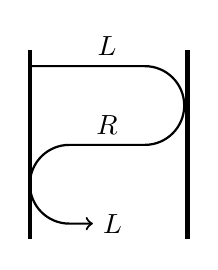
\begin{tikzpicture}
			\draw[ultra thick] (0,-1.2) -- (0,1.2);
			\draw[ultra thick] (2,-1.2) -- (2,1.2);
			\draw[->, thick] (0,1) -- (0.5,1) -- node[above] {$L$} (1.46, 1) arc  (90:-90:0.5) -- node[above] {$R$} (0.5,0) arc (-90:90:-0.5) -- (0.8,-1) node[right] {$L$};
		\end{tikzpicture}
		\caption{}
		\label{fig:reflections:aLL}
	\end{subfigure}
	\begin{subfigure}{.49\linewidth}
		\centering
		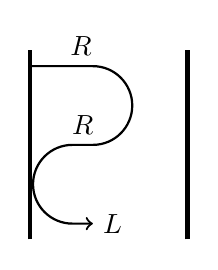
\begin{tikzpicture}
			\draw[ultra thick] (0,-1.2) -- (0,1.2);
			\draw[ultra thick] (2,-1.2) -- (2,1.2);
			\draw[->, thick] (0,1) -- (0.5,1) -- node[above] {$R$} (0.8, 1) arc  (90:-90:0.5) -- node[above] {$R$} (0.54,0) arc (-90:90:-0.5) -- (0.8,-1) node[right] {$L$};
		\end{tikzpicture}
		\caption{}
		\label{fig:reflections:aRL}
	\end{subfigure}
	\begin{subfigure}{.49\linewidth}
		\centering
		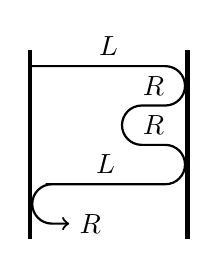
\begin{tikzpicture}
			\draw[ultra thick] (0,-1.2) -- (0,1.2);
			\draw[ultra thick] (2,-1.2) -- (2,1.2);
			\draw[->, thick] (0,1) -- (0.5,1) -- node[above] {$L$} (1.5, 1) -- (1.72,1) arc  (90:-90:0.25) -- node[above] {$R$} (1.42,0.5) arc (-90:90:-0.25) -- node[above]{$R$}(1.72,0) arc  (90:-90:0.25) -- node[above] {$L$} (0.2,-0.5)  -- (0.28,-0.5) arc (-90:90:-0.25) -- (0.5,-1) node[right]{$R$};
		\end{tikzpicture}
		\caption{}
		\label{fig:reflections:aLR}
	\end{subfigure}
	\begin{subfigure}{.49\linewidth}
		\centering
		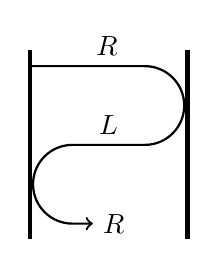
\begin{tikzpicture}
			\draw[ultra thick] (0,-1.2) -- (0,1.2);
			\draw[ultra thick] (2,-1.2) -- (2,1.2);
			\draw[->, thick] (0,1) -- (0.5,1) -- node[above] {$R$} (1.46, 1) arc  (90:-90:0.5) -- node[above] {$L$} (0.54,0) arc (-90:90:-0.5) -- (0.8,-1) node[right] {$R$};
		\end{tikzpicture}
		\caption{}
		\label{fig:reflections:aRR}
	\end{subfigure}
	\caption[Pathways in chiral medium]{The four pathways for a round-trip in a simple right-handed chiral cavity\cite{topf_modes_2014}. Reflections at interfaces with isotropic media are chirality reversing whereas distributed reflections are not. \ref{fig:reflections:aLL} Left-handed polarisation turned into left-handed polarisation. \ref{fig:reflections:aRL} Right-handed polarisation turned into left-handed polarisation. \ref{fig:reflections:aLR} Left-handed polarisation turned into right-handed polarisation. \ref{fig:reflections:aRR} Right-handed polarisation turned into right-handed polarisation.}
	\label{fig:reflections}	
\end{figure}

It has also been shown by \textcite{kopp_twist_2002}, \textcite{hodgkinson_supermodes_2003} and \textcite{oldano_comment_2004} that defect in a chiral photonic structure produces circularly polarised localised modes. Furthermore \textcite{harutyunyan_optical_2007} and \textcite{belyakova_optical_2011} showed that the orientation of such a defect layer in a chiral cavity allows switching handedness of the output and lowering the lasing threshold.
